\documentclass[tikz,border=10pt]{standalone}
\usepackage{tikz}
\usetikzlibrary{angles,quotes,calc}
\usepackage{tkz-euclide} %for right angle marker

\begin{document}
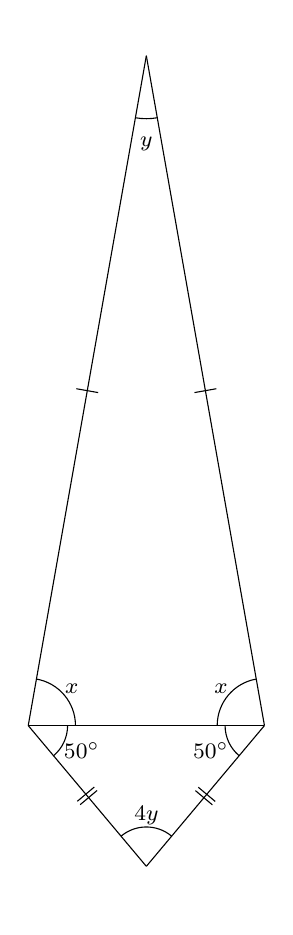
\begin{tikzpicture}[scale = 1]
    % Initial point
    \coordinate (D) at (0,0);
    % Draw base
    \draw (D) -- ++(0:3cm) coordinate (B);
    
    % % Draw triangle
    \path[name path=leg1] (D) -- ($(D)!3!80:(B)$) coordinate (K);
    \path[name path=leg2] (B) -- ($(B)!3!-80:(D)$) coordinate (L);
   
    \draw[name intersections={of=leg1 and leg2,by={A}}] (D) -- (A);
    \draw (B) -- (A);

     % Draw triangle 2
    \path[name path=leg3] (D) -- ($(D)!1!-50:(B)$) coordinate (N);
    \path[name path=leg4] (B) -- ($(B)!1!50:(D)$) coordinate (M);
    \draw[name intersections={of=leg3 and leg4,by={C}}] (D) -- (C);
    \draw (B) -- (C);

     \tkzMarkSegment[pos=.5,mark=|](D,A);
    \tkzMarkSegment[pos=.5,mark=|](B,A);
    \tkzMarkSegment[pos=.5,mark=||](C,B);
    \tkzMarkSegment[pos=.5,mark=||](D,C);
    
    % Draw the angle between lines
    \pic [draw, "\footnotesize $y$ ", angle eccentricity=1.4, angle radius=0.8cm] {angle = D--A--B};
    \pic [draw, "\footnotesize $x$", angle eccentricity=1.2, angle radius=0.6cm] {angle = A--B--D};
    \pic [draw, "\footnotesize $x$", angle eccentricity=1.2, angle radius=0.6cm] {angle = B--D--A};
    \pic [draw, "\footnotesize $50^\circ$ ", angle eccentricity=1.5, angle radius=0.5cm] {angle = C--D--B};
    \pic [draw, "\footnotesize $50^\circ$ ", angle eccentricity=1.5, angle radius=0.5cm] {angle = D--B--C};
    \pic [draw, "\footnotesize $4y$ ", angle eccentricity=1.3, angle radius=0.5cm] {angle = B--C--D};
   
\end{tikzpicture}
\end{document}

